\documentclass[a4paper,12pt]{ctexart}
\usepackage{../../teaching-style}

\begin{document}
\pagestyle{empty}

\maintitle{平面解析几何}
\begin{center}
  \large 高学段
\end{center}
\vspace{0.3cm}

\chaptertitle{第一章\quad 直线}

\sectiontitle{1.1\quad 直线的方程}

\knowbox{
\textbf{点斜式}：$y-y_0=k(x-x_0)$。\\
\textbf{斜截式}：$y=kx+b$。\\
\textbf{两点式}：$\dfrac{y-y_1}{y_2-y_1}=\dfrac{x-x_1}{x_2-x_1}$。\\
\textbf{截距式}：$\dfrac{x}{a}+\dfrac{y}{b}=1$。\\
\textbf{一般式}：$Ax+By+C=0$（$A,B$不全为$0$）。\\
\textbf{法线式}：$x\cos\alpha+y\sin\alpha-p=0$。}

\sectiontitle{1.2\quad 两直线的位置关系}

\knowbox{
平行：$k_1=k_2$且$b_1\neq b_2$，或$A_1B_2-A_2B_1=0$。\\
垂直：$k_1k_2=-1$，或$A_1A_2+B_1B_2=0$。\\
夹角：$\tan\theta=\left|\dfrac{k_2-k_1}{1+k_1k_2}\right|$。\\
点到直线距离：$d=\dfrac{|Ax_0+By_0+C|}{\sqrt{A^2+B^2}}$。}

\sectiontitle{习题1}

\begin{exercise}
\item 求过$(1,2)$且斜率$k=3$的直线方程。
\item 求过$(2,3)$和$(4,7)$的直线方程。
\item 两直线$l_1:y=2x+1$，$l_2:y=2x-3$是否平行？求它们之间的距离。
\item 求过$(1,-2)$且垂直于$3x-4y+5=0$的直线方程。
\item 求点$(2,3)$到直线$3x+4y-5=0$的距离。
\end{exercise}

\newpage

\chaptertitle{第二章\quad 圆}

\sectiontitle{2.1\quad 圆的方程}

\knowbox{
\textbf{标准方程}：$(x-a)^2+(y-b)^2=r^2$，圆心$(a,b)$，半径$r$。\\
\textbf{一般方程}：$x^2+y^2+Dx+Ey+F=0$（$D^2+E^2-4F>0$）。\\
圆心$\left(-\dfrac D2,-\dfrac E2\right)$，半径$r=\dfrac12\sqrt{D^2+E^2-4F}$。}

\sectiontitle{2.2\quad 直线与圆的位置关系}

\knowbox{
$d<r\Leftrightarrow$相交（两个交点）；\\
$d=r\Leftrightarrow$相切（一个交点）；\\
$d>r\Leftrightarrow$相离（无交点）。\\
弦长公式：$|AB|=2\sqrt{r^2-d^2}$。\\
圆的切线：过圆上一点$(x_0,y_0)$的切线为$(x_0-a)(x-a)+(y_0-b)(y-b)=r^2$。\\
圆的幂：$P$对圆$\odot O$的幂$=PO^2-r^2$。}

\sectiontitle{习题2}

\begin{exercise}
\item 求圆心$(2,-3)$半径$4$的圆的方程。
\item 判断点$(1,2)$与圆$(x-1)^2+(y+1)^2=9$的位置关系。
\item 求$2x-3y+1=0$与圆$x^2+y^2=5$的交点个数。
\item 求过$(3,4)$且与圆$x^2+y^2=25$相切的切线方程。
\end{exercise}

\newpage

\chaptertitle{第三章\quad 圆锥曲线}

\sectiontitle{3.1\quad 椭圆}

\knowbox{
定义：到两焦点距离之和为常数$2a$。\\
标准方程：$\dfrac{x^2}{a^2}+\dfrac{y^2}{b^2}=1$（$a>b>0$）。\\
$a$长半轴，$b$短半轴，$c=\sqrt{a^2-b^2}$。\\
离心率$e=\dfrac ca<1$。\\
焦点$(\pm c,0)$，顶点$(\pm a,0)$、$(0,\pm b)$。}

\begin{center}
\begin{tikzpicture}[scale=0.6]
\draw[thick] (0,0) ellipse (3 and 2);
\draw[->,thick] (-3.5,0) -- (3.5,0) node[right] {$x$};
\draw[->,thick] (0,-2.5) -- (0,2.5) node[above] {$y$};
\filldraw (-2.236,0) circle (2pt) node[below] {$F_1(-c,0)$};
\filldraw (2.236,0) circle (2pt) node[below] {$F_2(c,0)$};
\node at (3,1.5) {$\dfrac{x^2}{a^2}+\dfrac{y^2}{b^2}=1$};
\end{tikzpicture}
\end{center}

\sectiontitle{3.2\quad 双曲线}

\knowbox{
定义：到两焦点距离之差的绝对值为常数$2a$。\\
标准方程：$\dfrac{x^2}{a^2}-\dfrac{y^2}{b^2}=1$。\\
$c=\sqrt{a^2+b^2}$，离心率$e=\dfrac ca>1$。\\
渐近线：$y=\pm\dfrac ba x$。}

\sectiontitle{3.3\quad 抛物线}

\knowbox{
定义：到焦点距离等于到准线距离。\\
标准方程$y^2=2px$：焦点$(\dfrac p2,0)$，准线$x=-\dfrac p2$。\\
离心率$e=1$。}

\sectiontitle{3.4\quad 直线与圆锥曲线的位置关系}

\knowbox{
联立方程$\rightarrow$判别式法：\\
$\Delta>0$相交，$\Delta=0$相切，$\Delta<0$相离。\\
弦长公式：$|AB|=\sqrt{1+k^2}|x_1-x_2|$或$\sqrt{1+\dfrac1{k^2}}|y_1-y_2|$。\\
韦达定理的应用：中点弦、弦中点轨迹。}

\sectiontitle{习题3}

\begin{exercise}
\item 椭圆$\dfrac{x^2}{25}+\dfrac{y^2}{9}=1$，求$a,b,c,e$和焦点坐标。
\item 双曲线$\dfrac{x^2}{16}-\dfrac{y^2}{9}=1$，求$a,b,c$和渐近线方程。
\item 抛物线$y^2=8x$，求焦点坐标和准线方程。
\item 求直线$y=x+1$与椭圆$\dfrac{x^2}{4}+y^2=1$的交点个数。
\item 求过焦点且垂直于$x$轴的直线被抛物线$y^2=4x$截得的弦长。
\end{exercise}

\newpage

\chaptertitle{第四章\quad 轨迹方程与坐标变换}

\sectiontitle{4.1\quad 轨迹方程的求法}

\knowbox{
1. 直接法：根据几何条件直接列方程。\\
2. 定义法：利用圆锥曲线定义。\\
3. 代入法（相关点法）：$P$随$Q$运动，已知$Q$轨迹求$P$轨迹。\\
4. 参数法：引入参数表示坐标，消参得到方程。\\
5. 交轨法：求两动直线交点的轨迹。}

\sectiontitle{4.2\quad 极坐标与参数方程}

\knowbox{
\textbf{极坐标}$(\rho,\theta)$，$\rho\ge0$，$0\le\theta<2\pi$。\\
与直角坐标关系：$x=\rho\cos\theta$，$y=\rho\sin\theta$；$\rho^2=x^2+y^2$，$\tan\theta=\dfrac yx$。\\
\textbf{参数方程}：\\
直线$\begin{cases}x=x_0+t\cos\alpha\\y=y_0+t\sin\alpha\end{cases}$（$t$为参数）。\\
圆$\begin{cases}x=a+r\cos\theta\\y=b+r\sin\theta\end{cases}$。\\
椭圆$\begin{cases}x=a\cos t\\y=b\sin t\end{cases}$。\\
抛物线$\begin{cases}x=2pt^2\\y=2pt\end{cases}$。}

\sectiontitle{习题4}

\begin{exercise}
\item 求到$(2,0)$和$(-2,0)$距离之和为$6$的点的轨迹方程。
\item 点$P$在圆$x^2+y^2=4$上运动，$M$为$P$与点$(3,0)$的中点，求$M$的轨迹。
\item 化直角坐标$x^2+y^2=4x$为极坐标方程。
\item 求椭圆$\dfrac{x^2}{9}+\dfrac{y^2}{4}=1$的参数方程。
\item 求直线$\begin{cases}x=2+t\\y=1-t\end{cases}$与曲线$\begin{cases}x=2\cos\theta\\y=\sin\theta\end{cases}$的交点坐标。
\end{exercise}

\newpage
\sectiontitle{参考答案}

\subsection*{习题1}
\begin{enumerate}
  \item $y=3x-1$
  \item $y=2x-1$
  \item 平行，距离$d=\dfrac{4\sqrt5}{5}$
  \item $4x+3y+2=0$
  \item $\dfrac{13}{5}$
\end{enumerate}

\subsection*{习题2}
\begin{enumerate}
  \item $(x-2)^2+(y+3)^2=16$
  \item 点在圆上
  \item $2$个交点
  \item $3x+4y-25=0$
\end{enumerate}

\subsection*{习题3}
\begin{enumerate}
  \item $a=5$，$b=3$，$c=4$，$e=\dfrac45$，焦点$(\pm4,0)$
  \item $a=4$，$b=3$，$c=5$，渐近线$y=\pm\dfrac34x$
  \item 焦点$(2,0)$，准线$x=-2$
  \item $2$个交点
  \item 弦长$4$
\end{enumerate}

\subsection*{习题4}
\begin{enumerate}
  \item $\dfrac{x^2}{9}+\dfrac{y^2}{5}=1$
  \item $\bigl(x-\dfrac32\bigr)^2+y^2=1$
  \item $\rho=4\cos\theta$
  \item $\begin{cases}x=3\cos t\\y=2\sin t\end{cases}\;(t\in[0,2\pi))$
  \item 无交点
\end{enumerate}

\end{document}
